\documentclass[a4paper,11pt]{article}
\usepackage{graphicx}
\usepackage{hyperref}

\begin{document}
\begin{center}

\Huge\textbf{Functional Requirements\\}
																											
\vspace{2 cm}

\LARGE\textbf{Group Name:} Group 6\_b\newline
 
\vspace{0.5 cm}
\begin{tabular}{lr}
Jessica (JI) Lessev&13049136\\
Thabang (TM) Letageng&13057937\\
Michelle Swanepoel&13066294\\
Prenolan Govender&13102380\\
Fako (FJA) Peleha&12230830\\
Lutfiyya Razak&10198408\\
Ephiphania Munava&10624610\\
Maria Qumalo&29461775\\
\end{tabular}

\vspace{1cm}
\textbf{Git repository link:\\}
\url{https://github.com/u12230830/COS301\_6b}

\vspace{1cm}
\textbf{Date:} 27 February 2015
\end{center}




\newpage

%Section Functional requirements
\begin{center}
\huge\section{Functional Requirements}
\end{center}

\subsection{Use case prioritization}
Jessica and Michelle\\
Jimmy\\
Ephi\\
\textbf{Critical}: Management of user profiles.
Thabang\\
\\
Prenolan\\
\textbf{Important}: Voting on and evaluation of posts.
\\
\textbf{Nice-To-Have}: Marking a post as the best answer.
\\
\\
Lutfiyya\\
\textbf{Important}: Evaluation Report
\\
\\
Maria\\


\subsection{Use case/ Services contracts}
Jessica and Michelle\\
Jimmy\\
Ephi\\
\subsubsection{Managing User Profile}
\textbf{Pre-Condition}: A user must be a registered member of the university and a registered member of one or more modules available on the BuzzSpace.
\\
\textbf{Post-Condition}: The user is registed and can now login thus it is now possible for the user to comment, tag and vote for threads on the BuzzSpace. The user now has a profile on the BuzzSpce meaning the can have a status, thus enabling diffent functionality at different status levels.
\\
\\
\includegraphics{Images/ManageUserProfile/Class_Diagram_Input}
\includegraphics{Images/ManageUserProfile/Class_Diagram_Output}
\\
Thabang\\
\\
Prenolan
\subsubsection{Voting and Evaluation}
\textbf{Pre-Condition}: A post has to have been created for a user to be able to vote on or evaluate it. Any user can vote on or evaluate a post as long as the user is logged in and a part of a specific Buzz Space. An exception to this rule is when the administration of a Buzz Space set specific rules as to which users (perhaps based on status) can vote on or evaluate posts.
\\
\textbf{Post-Condition:} A vote or evaluation has to be visible to every user (or only some based on the administration of that space) after it has been made on a post. A positive vote or evaluation has to reflect upon the posters progress to the next status level.
\\
\\
\includegraphics{Images/VotesAndEvaluation/Class_Diagram__Input}
\includegraphics{Images/VotesAndEvaluation/Class_Diagram__Output}
\\
\subsubsection{Best Answer}
\textbf{Pre-Condition}: A user must have the privileges set by the administration of a space in order to mark a post as the best answer. The user is required to be logged in.
\\
\textbf{Post-Condition}: The thread should effectively display that an answer has been selected and optionally close the thread. The poster of the best answer should acquire an increase in progress to the next status level.
\\
\\
\includegraphics{Images/BestAnswer/Class_Diagram}
\\
\\
Lutfiyya\\
\subsubsection{Evaluation Report}
\textbf{Pre-Condition}: A lecturer has to be a registered user of a Buzz Space and must also be logged in to be able to generate an evaluation report of the students. The UserID of a participant should exist for reporting purposes.
\\
\textbf{Post-Condition:} A lecturer should get statistical information about each student and generate an evaluation report for a participant
\\
\\
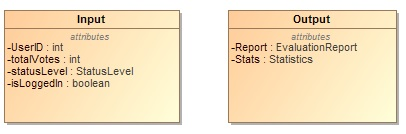
\includegraphics{Images/Report/Input&Output}
\\
\\
Maria\\

\subsection{Required functionality}
Jessica and Michelle\\
Jimmy\\
Ephi\\
\begin{center}
\includegraphics[width=0.9\linewidth]{./Images/ManageUserProfile/functional_requirements}
\end{center}
Thabang\\
Prenolan\\
\begin{center}
\includegraphics[width=0.9\linewidth]{./Images/VotesAndEvaluation/functional_requirements}
\end{center}

\begin{center}
\includegraphics[width=0.9\linewidth]{./Images/BestAnswer/functional_requirements}
\end{center}

Lutfiyya\\
\includegraphics[width=15cm,height=10cm]{./Images/Report/functional_requirements}\\
\\

Maria\\

\subsection{Process specification}
Jessica and Michelle\\
Jimmy\\
Ephi\\

\begin{center}
\includegraphics[width=0.9\linewidth]{./Images/ManageUserProfile/functional_requirements}
\end{center}

Thabang\\
Prenolan\\
\begin{center}
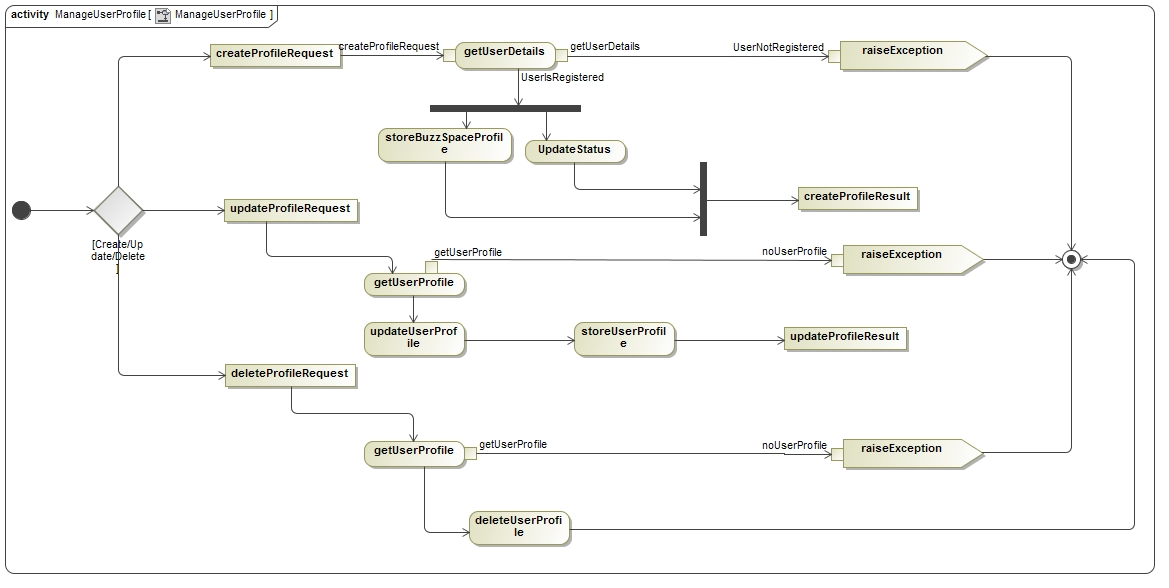
\includegraphics[width=0.9\linewidth]{./Images/VotesAndEvaluation/process_specification}
\end{center}

\begin{center}
\includegraphics[width=0.9\linewidth]{./Images/BestAnswer/process_spec}
\end{center}

Lutfiyya\\
%\begin{figure}
%\centering
\includegraphics[width=15cm,height=10cm]{./Images/Report/process_spec}
%\caption{Process specification for evaluation of reports}
%\end{figure}

Maria\\

\subsection{Domain model}


\end{document}

